\chapter{Introduction to Proof Complexity}

Up to this point we have  seen \textbf{circuit complexity}, in which we wished to understand the resources required to \emph{compute} a function. And specifically, what is the minimal size of a Boolean circuit computing a given function (as a function of the number of input bits).

We now consider \textbf{proof complexity}. Instead of analysing the size of circuits computing Boolean
functions, we address the question:



\bigskip

\noindent
\hangindent=2em
\hangafter=0
Given a propositional proof system, and a tautological
statement (valid statement; namely a propositional
formula that is 1 under any assignment), what is the
shortest proof of this statement?

\bigskip


Like circuit complexity was motivated by $\P$ vs $\NP$ (if SAT
does not have small circuits then $\P \neq \NP$), proof
complexity is motivated by the $\NP$ vs $\coNP$ question.


% Do not use float option, otherwise it's not put inline. 
\begin{tcolorbox}[colframe=white, colback=gray!5, boxrule=0mm, sharp corners]
\textbf{Recall some basic notions from complexity classes.
}

\textbf{NP}: all languages with polynomial-size witnesses. \\
\textbf{coNP}: all languages whose \textit{negative} instances have
polynomial-size witnesses.

Formally:





$L \in NP$: There is a relation $R(\bar{x}, \bar{y})$ in $P$ and a constant $C$, such that $x \in L$ iff 
\[ \exists \bar{y} (|\bar{y}| \leq |\bar{x}|^C \land R(\bar{x}, \bar{y}) = 1). \]

$L \in coNP$: Let 
\[ \bar{L} = \{ x \in \{0,1\}^* \mid x \notin L \}. \]
Then $L \in coNP$ iff $\bar{L} \in NP$.

In other words, there is a relation $R(\bar{x}, \bar{y})$ in $P$ and a constant $C$, such that $x \in L$ iff 
\[ \forall \bar{y} (|\bar{y}| \leq |\bar{x}|^C \to R(\bar{x}, \bar{y}) = 0). \]

For concreteness, we can think of $NP, coNP$ as:
\begin{align*}
    SAT \text{ as }  NP \\
    UNSAT \text{ as } coNP
\end{align*}

\text{Given a CNF formula, given a CNF formula,}

\text{accept if there exists accept if there is no}

\text{a satisfying assignment satisfying assignment.}

Indeed: 
\begin{align*}
    SAT &\text{ is NP-complete, hence,} \\
    UNSAT &\text{ is coNP-complete.}
\end{align*}

\begin{itemize}
    \item For language $L$ in NP, we know we have short (polynomial-size) proofs for every $x$ in $L$: if $L = SAT$, then the short proof is simply the satisfying assignment.
    \item For language $L$ in coNP, we don't know if $x$ in $L$ have short proofs. If $L = UNSAT$, and $x$ is in $L$, then what kind of short proofs are there for unsatisfiability? It's open if there are!
    \item To study this question we investigate proofs in different proof systems (like circuits in different circuit classes).
\end{itemize}

\end{tcolorbox}


%%%%%%%%%%%%%%%%%%%%%%%%%%%%%%%%%%%%%%%%%%%%
\section{The Resolution Refutation  System} 
%%%%%%%%%%%%%%%%%%%%%%%%%%%%%%%%%%%%%%%%%%%%

For the rest of this chapter we focus on a  concrete proof system, which is well studies, simple to describe, and quite well-understood. 


\begin{tcolorbox}[colframe=white, colback=red!5, boxrule=0mm, sharp corners]
\textbf{Resolution Refutations}
\begin{itemize}
    \item Let $F$ be an unsatisfiable set of  clauses $C_1, \dots, C_m$.
    \item A \textit{resolution refutation} of $F$ is a sequence of clauses $D_1, \dots, D_t$ such that $D_t = \square$ (the empty clause, which stands for the true value false), and every $D_i$ is either $C_i$ for some $i=1,\dots,m$, or was derived from $D_j, D_k$ with $j,k < i$ via the resolution derivation rule:
\end{itemize}

\textbf{Resolution Rule:}
\begin{center}
    \begin{tabular}{c}
        \hline
        From $A \lor x$ and $B \lor \neg x$ \\
        Derive $A \lor B$ \\
        \hline
    \end{tabular}
\end{center}

Where $A, B$ are some clauses themselves.

\textbf{Weakening Rule:}
\begin{center}
    \begin{tabular}{c}
        \hline
        From $A$ (a clause) \\
        Derive $A \lor l$ ($l$ a literal) \\
        \hline
    \end{tabular}
\end{center}

The \textbf{size} of a resolution refutation is the number of clauses it has.
\end{tcolorbox}

\begin{figure}[H]\label{fig:res-refutation}
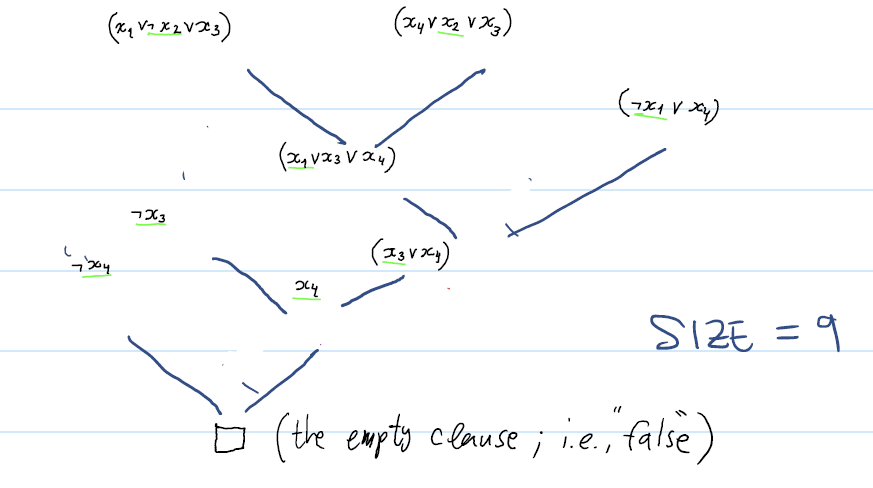
\includegraphics{images/resolution-example.png}
\caption{Example of a resolution refutation depicted as a tree whose labels are clauses.}
\end{figure}
As a sequence of clauses, we can depict the refutation in Figure \ref{fig:res-refutation} as follows:


\[
\begin{array}{ll}
1. & x_1 \vee x_2 \vee x_3 \quad \text{(Axiom)} \\
2. & x_4 \vee x_2 \vee x_3 \quad \text{(Axiom)} \\
3. & x_1 \vee x_2 \vee x_3 \vee x_4 \quad \text{(Derived from 1, 2)} \\
4. & x_1 \vee x_2 \vee \neg x_4 \quad \text{(Axiom)} \\
5. & x_1 \vee x_3 \quad \text{(Derived from 4, 3)} \\
6. & x_3 \vee x_4 \quad \text{(Axiom)} \\
7. & x_3 \quad \text{(Derived from 5, 6)} \\
8. & x_1 \quad \text{(Axiom)} \\
9. & \text{False} \quad \text{(Derived from 7, 8).}
\end{array}
\]

% 
% \begin{align*}
%     & x_1 \lor x_2 \lor x_3, \quad x_4 \lor x_2 \lor x_3, \quad x_1 \lor x_2 \lor \neg x_4, \quad x_1 \lor x_3, \quad x_3 \lor x_4, \\
%     & x_3, \quad x_1, \quad \text{False} \\
% \end{align*}
% where going from left to right, the following are the axioms and derivation rules applies:
% \begin{itemize}
%     \item $1,2$ (axioms)
%     \item Derive from $1,2$
%     \item Axiom
%     \item Derive from $4,3$
%     \item Axiom
%     \item Derive from $5,6$
%     \item Axiom
%     \item Derive from $7,8$
% \end{itemize}

\textbf{Comments:} The example depicted a \textbf{tree-like} resolution refutation because the underlying structure is a \textbf{tree}. Formally, this means that every clause in the refutation is used at most once in a resolution rule (to derive a new clause). Hence, the underlying structure of the proof can be drawn as a \textbf{tree}.

A resolution refutation that is \textbf{not} a tree, namely, the same occurrence of a clause can be used in more than one resolution-rule applications, is called a \textbf{DAG-like refutation}. Because the refutation can be drawn as a \textbf{Directed Acyclic Graph}.


\textbf{Comment:} We use the word "proof" and "refutation" interchangeably in proof complexity.

A refutation of a CNF is a proof that it is unsatisfiable. Or in other words, a proof that the negation of the CNF is a tautology, i.e., evaluates to 1 under any assignment.


We need the following simple definitions and notations to explain the completeness of the resolution refutation system.

For a variable $x$ we define $x^1 := x$ and $x^0 := \neg x$.
 

\begin{definition}[Restriction of a proof/refutation]
Let $F$ be a CNF.
Define $F\rst_{x_i := \epsilon}$, $\epsilon \in \{0,1\}$ as follows:
For all clauses $C$ in $F$ do:
\begin{enumerate}
    \item If $C$ is a clause in $F$ and $x_i^\epsilon \in C$, then delete $C$ from $F$.
    \item If $x_i^{1-\epsilon} \in C$, then delete the literal $x_i^{1-\epsilon}$ from $C$ (keep $C$).
    \item Otherwise, do nothing.
\end{enumerate}
\end{definition}

\textbf{Examples:}
\begin{enumerate}
    \item $(x_1 \lor x_2 \lor x_3)$  
    \[
    F\rst_{x_1 := 0} \Rightarrow (x_2 \lor x_3)
    \]

    \item $(x_1 \lor x_2 \lor \neg x_3)$  
    \[
    F\rst_{x_1 := 1} \Rightarrow (1\lor x_2 \lor \neg x_3)\equiv 1
    \]
    (Delete this clause  because it is not usable in a refutation).
\end{enumerate}

\textbf{Conclusion:}  
$F\rst_{x := \epsilon}$ for $\epsilon \in \{0,1\}$ is simply assigning $0,1$ in $F$ for $x$, where $0,1$ then leads to deletion of literal or clause, respectively.




\begin{theorem}
Resolution is a complete refutation system for unsatisfiable CNF formulas. In other words, every unsatisfiable CNF formula has a resolution refutation. 
\end{theorem}

\begin{proof}
Let $F$ be a CNF formula that is unsatisfiable. This means that $F$ evaluates to false (or 0) under every truth assignment to the variables of $F$. Our goal is to show that the empty clause (denoted as $\square$) can be derived using resolution.

We construct a resolution refutation by induction on the number of variables $n$.

\Base $F$ contains one variable. 
If $F$ contains just one variable, say $x_1$, and is unsatisfiable, then it must contain both $x_1$ and $\neg x_1$ as clauses (each with a single literal).
Resolving these two immediately yields the empty clause $\square$.

\induction  Assume that resolution is complete for CNFs with $n$ variables.
    \item Now, consider a CNF $F$ with $n+1$ variables.
    \item We perform a ``splitting method'' by considering:
    \begin{itemize}
        \item $F[x_{n+1}=1]$, the simplified formula when $x$ is set to true.
        \item $F[x_{n+1}=0]$, the simplified formula when $x$ is set to false. Since $F$ is unsatisfiable, both $F[x_{n+1}=1]$ and $F[x_{n+1}=0]$ must also be unsatisfiable.
        \item By the induction hypothesis, there exist resolution refutations for both. We can \emph{glue} these refutations into one, as is shown in the Gluing Lemma below eventually leading to $\square$.
    \end{itemize}
 
  
 
 

\begin{lemma}[The glueing lemma]
\label{lem:glueing-no-width}
The resolution refutation of $F_{x_i := 0} \vdash \square$ and the resolution refutation of $F_{x_i := 1} \vdash \square$ can be glued together into a refutation of $F$.

\end{lemma}
This suffices for our proof of completeness, when we put $i = n+1$.


\para{Upshot of the argument}

We construct from a refutation of $F\!\rst_{x_i=0}$ a derivation of $x_i$ from $F$. We then use this derivation, namely the clause $x_i$, to cut all occurrences of $\neg x_i$ from $F$. By cutting $\neg x_i$ from $F$ we get $F\!\rst_{x_i=1}$, because $F\!\rst_{x_i=1}$ contains precisely all clauses $C$ such that $\neg x\lor C$ in $F$ and all clauses $D$ that neither contain $x_i$ nor $\neg x_i$ (clauses $x_i\lor E$ in $F$ are discarded from $F$ when we assign $x_i=1$). By induction hypothesis we know that  $F\!\rst_{x_i=1}$ has a resolution refutation and we are finished.


\begin{figure}[H]
    \centering
    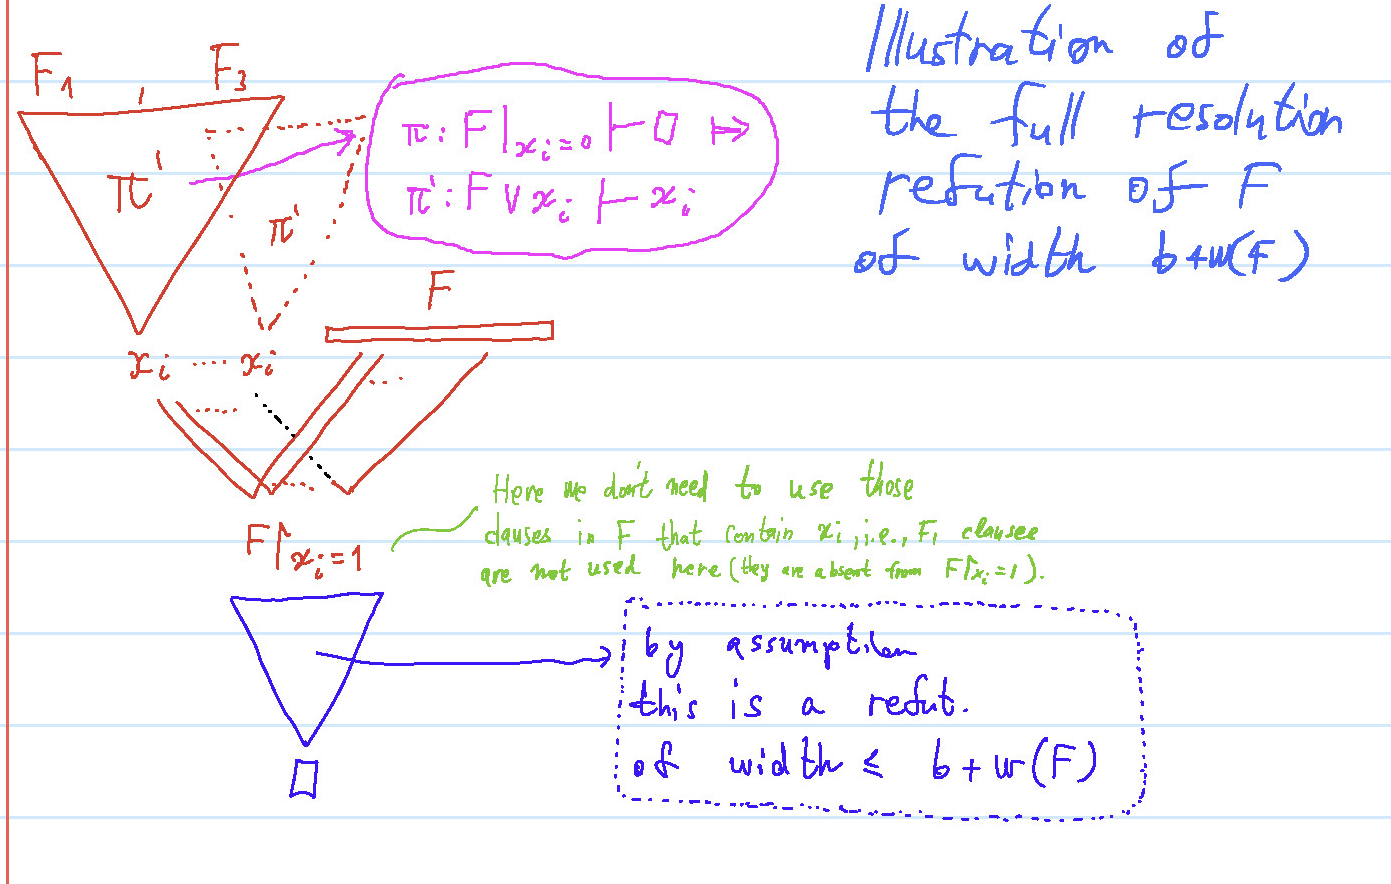
\includegraphics[width=\textwidth]{images/second-glueing-illustration.png}
    \caption{An illustration of the glueing lemma. }
    \label{fig:pluck-stage}
\end{figure}


%Using induction assumption, we construct from a refutation of $F\!\rst_{x_i=0}$ a derivation of $x_i$ from $F$. We then use this derivation, namely the clause $x_i$, to cut all occurrences of $\neg x_i$ from $F$. By cutting $\neg x_i$ from $F$ we get $F\!\rst_{x_i=1}$, because $F\!\rst_{x_i=1}$ contains precisely all clauses $C$ such that $\neg x\lor C$ in $F$ and all clauses $D$ that neither contain $x_i$ nor $\neg x_i$ (clauses $x_i\lor E$ in $F$ are discarded from $F$ when we assign $x_i=1$). By induction hypothesis we know that  $F\!\rst_{x_i=1}$ has a resolution refutation and we are finished.


\begin{proof}
Assume $F_{x_i := 0} \vdash \square$, meaning that we have a resolution refutation of $F_{x_i := 0}$.

Then, $F \vdash x_i$, meaning there is a resolution derivation of $x_i$ from $F$.
  

Consider $F_{x_i := 0} \vdash \square$.

- We are going to turn this refutation from $F_{x_i := 0}$ to a \textbf{derivation} of $x_i$ from $F$.

  This is done by, roughly, adding OR of $x_i$ to each clause in the refutation $F_{x_i := 0} \vdash \square$.

- How do we do this precisely?  
  Consider three types of clauses in $F$:

  1) \textbf{Clauses containing literal $x_i$:}  
     We denote this set of clauses by $F_1$.

  2) \textbf{Clauses containing literal $\neg x_i$:}  
     We denote this set of clauses by $F_2$.  
     ($F_1$ is disjoint from $F_2$, because we assume we don’t have clauses of the form $C' \lor x_i \lor \neg x_i$, since we can get rid of such clauses without increasing the size).

  3) \textbf{Clauses without $x_i$ and without $\neg x_i$:}  
     We denote this set of clauses by $F_3$.
```
 

Now consider what happens to $F = F_1 \cup F_2 \cup F_3$ when we assign $x_i = 0$ in $F_{x_i := 0}$:

\begin{enumerate}
    \item A clause in $F_1$ looks like $x_i \lor D$.
    \begin{itemize}
        \item So in $F_{x_i := 0}$, it turns into $D$.
    \end{itemize}

    \item A clause in $F_2$ contains $\neg x_i$.
    \begin{itemize}
        \item So in $F_{x_i := 0}$, this clause becomes True and is erased.
    \end{itemize}

    \item A clause in $F_3$ does not contain the variable $x_i$, so in $F_{x_i := 0}$ it stays the same.
\end{enumerate}

Now we are ready to convert $F_{x_i := 0} \vdash \square$ to $F \vdash x_i$ (i.e., a derivation of the clause $x_i$ from $F$).

\textbf{Idea:}

\begin{center}
\textit{Simply add} $ \lor x_i$ \textit{to each clause in} $F_{x_i := 0} \vdash \square$.
\end{center}
 

It remains to show that doing so turns  
$F_{x_i := 0} \vdash \square$ into $F \vdash x_i$.

\begin{enumerate}
    \item A clause $D$ in $F_{x_i := 0}$ was the clause $D \lor x_i$ in $F$,
    
    \begin{itemize}
        \item which when assigning $x_i = 0$ turned into $D$. Now, when we add $\lor x_i$, we get back to the original clause $D \lor x_i$ in $F$.
    \end{itemize}

    \item A clause $D \lor \neg x_i$ in $F_2$ has disappeared in $F_{x_i := 0}$, so it doesn’t appear in $F_{x_i := 0} \vdash \square$.

    \item A clause $D$ in $F_3$ does not contain $x_i$ or $\neg x_i$. When we add $\lor x_i$ to $D$, we get a new clause not in $F$.
    
    \begin{itemize}
        \item But we can derive, using a single \textbf{Weakening Rule}, the clause $D \lor x_i$.  
        \item Hence, in every place $D \lor x_i$ appears, we simply add $D$ to the resolution derivation, which turns it into a legal resolution derivation from $F$.
    \end{itemize}
\end{enumerate}

 

\begin{enumerate}
    \item[e)] If in $F_{x_i := 0} \vdash \square$ we used the resolution rule:
    \[
    \frac{A \lor u}{A \lor B} \quad \frac{B \lor w}{A \lor B}
    \]
    for some variable $w \in \{x_1, \dots, x_n\} \setminus \{x_i\}$  
    (\textit{recall that variable $x_i$ doesn't occur in} $F_{x_i := 0}$),  
    then when adding $\lor x_i$, it turns into a \textbf{legit} resolution rule:

    \[
    \frac{
    x_i \lor A \lor x_j \qquad x_i \lor B \lor \neg x_j}{    x_i \lor A \lor B
 }   \]

    \hfill $\square$ (Claim)
\end{enumerate}

\textbf{Illustration of the transformation from $F$ to $F_{x_i := 0}$}

\begin{center}
\begin{tabular}{c c c}
    $x_i \in F_1$ & $x_i \in F_2$ & $x_i, \neg x_i \notin F$ \\
    $(x_i \lor D_1), (x_i \lor D_2)$ & $(\neg x_i \lor C_1), (\neg x_i \lor C_2)$ & $F_3$ \\
    Original $F$ & Original $F$ & $F_{x_i := 0}$ \\
    $D_1, \dots, D_k$ & & $F_3$ \\
    $F_1$ & & $F_3 \lor x_i$ (weakening) \\
\end{tabular}
\end{center}

By the claim, we get a resolution derivation $\pi$ of $x_i$ from $F$.
 

- Now, we use $F \vdash x_i$ on the clauses of $F$ to get rid (resolve) all the literals $\neg x_i$ in $F$.

  This is simple: derive $x_i$ from $F$, and then resolve $D \lor \neg x_i$ in $F$ by $x_i$ to get $D$.

- Note that this way we got a derivation of $F_{x_i := 1}$ from $F$.

  This is because $F_{x_i := 1}$ contains precisely all the clauses in $F$ that contain neither $x_i$ nor $\neg x_i$ ($F_3$ above), and the clauses $D$ such that $x_i \lor D$ is in $F$ (i.e., $F_2$ above).  
  (The clause $x_i \lor D$ in $F$ gets deleted in $F_{x_i := 1}$.)

 
By assumption $F_{x_i := 1} \vdash \square$, namely, after we derived $F_{x_i := 1}$ from $F$ with a resolution derivation, we derive $\square$, and finish the proof of the glueing lemma.
\end{proof} % Gluing lemma
\end{proof} % completeness of resolution 
 
%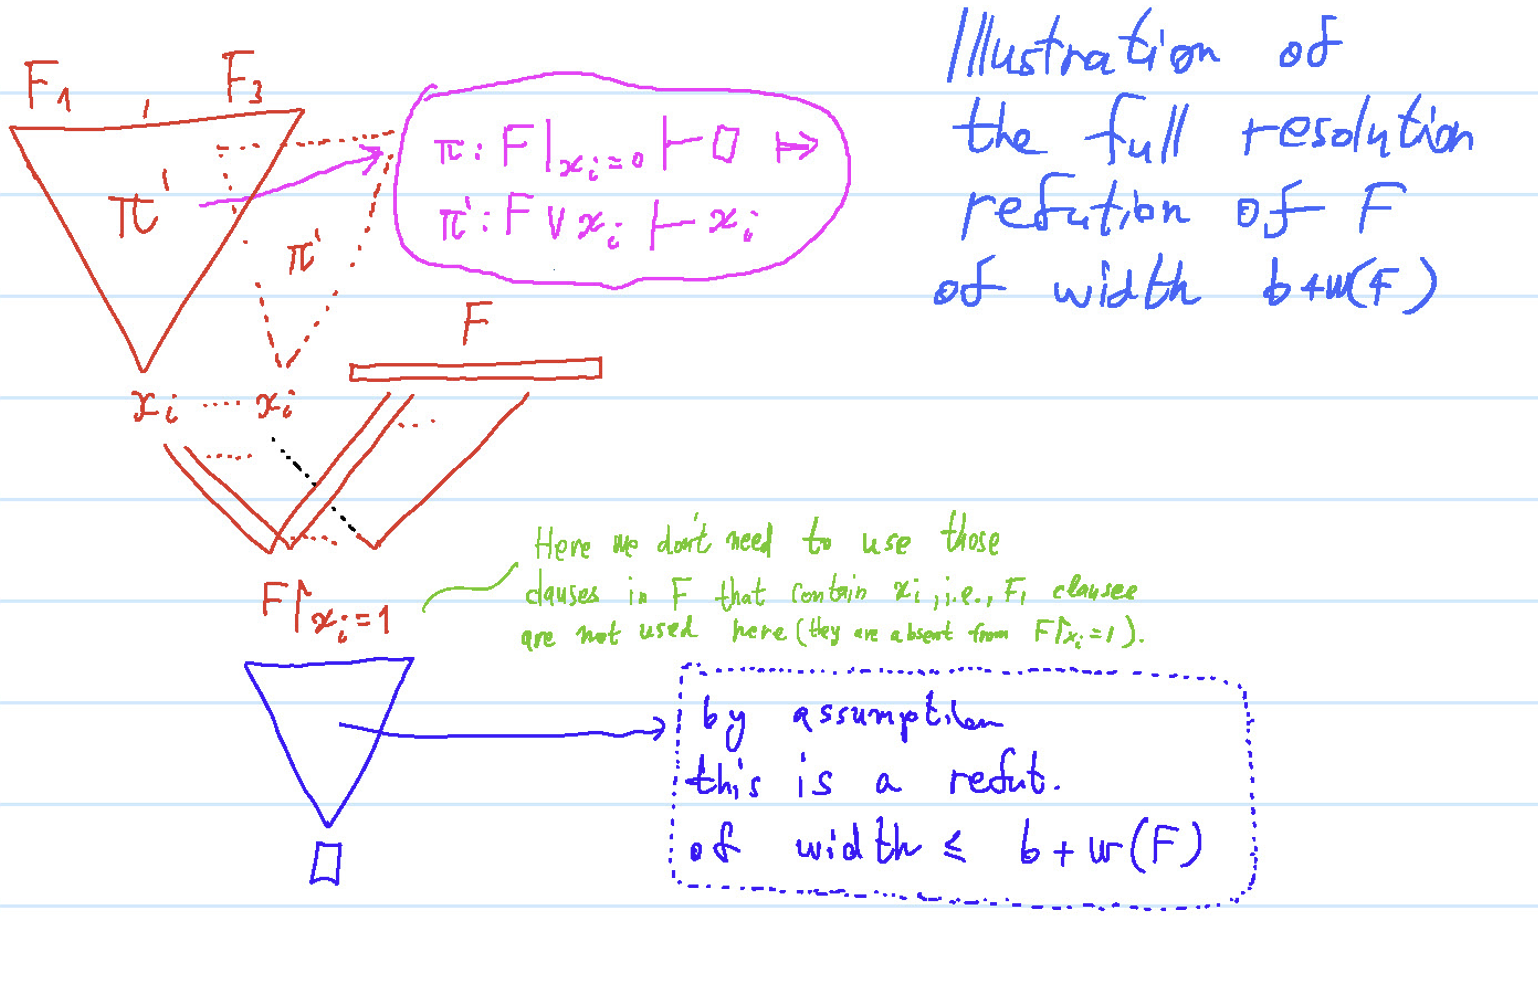
\includegraphics[width=\textwidth]{image015.png}


\section{Abstract Propositional Proof Systems}

\begin{definition}[Propositional Proof System]
A propositional proof system is a polynomial-time algorithm $A(\tau, \pi)$ with two inputs:  
- A tautology $\tau$ (a propositional formula that is satisfied by every assignment) or equivalently an unsatisfiable propositional formula,  
- Such that:  
\[
\exists \pi \in \Sigma^* (A(\tau, \pi) = 1) \text{ iff } \tau \text{ is a tautology}.
\]
\end{definition}

\textbf{Important note:} $A(\tau, \pi)$ is a poly-time algorithm for checking the \textbf{correctness} of the proof $\pi$ of $\tau$.

- The runtime of $A$ is \textbf{not} polynomially bounded in the size of $\tau$, rather in the size of \textbf{both} $\tau$ and its proof $\pi$!
- It might happen that some tautologies $\tau$ do not have proofs $\pi$ with size polynomial in $\tau$ in any propositional proof system (that’s open! And would imply $P \neq NP$).

\textbf{Intuition} behind the definition of propositional proof systems:
- A "proof" is something that can be \textbf{easily checked} once given.
- "Easily" in computational complexity means polynomial-time.
- Make sure that you understand the following distinction:
  \begin{enumerate}
      \item Checking the correctness of a given proof $\pi$.
      \item Finding a proof $\pi$ given $\tau$.
  \end{enumerate}


We use the following terminology:

\textbf{Completeness:} A propositional proof system is complete because if $\tau$ is a tautology, then there exists a proof $\pi$.  
That is, \textbf{all} tautologies have proofs.

\textbf{Soundness:} A propositional proof system is sound because if $\tau$ has a proof, then $\tau$ is a tautology.  
That is, \textbf{only} tautologies have a proof.

Similar to circuit complexity, we consider the \textbf{asymptotic behavior} of proof systems:

A \textbf{family} of tautologies $\{\tau_n\}_{n=1}^{\infty}$ is a collection of propositional formulas $\tau_n$ such that $\tau_n$ is a tautology with $n$ variables for all $n \in \mathbb{N}$.

Similarly, we consider a \textbf{family} of proofs for $\{\tau_n\}_{n=1}^{\infty}$.

Let $P$ be a propositional proof system.

A \textbf{family} of $P$-proofs $\{\pi_n\}_{n=1}^{\infty}$ of the family of tautologies $\{\tau_n\}_{n=1}^{\infty}$ is a collection of $P$-proofs, such that $\pi_n$ is a $P$-proof of $\tau_n$ for all $n \in \mathbb{N}$ (with $n$ being the number of variables in $\pi_n$ and $\tau_n$).

\begin{definition}
A family of tautologies $\{\tau_i\}_{i=1}^{\infty}$ has \textbf{polynomial-size proofs} in a propositional proof system $P$, if there exists a family $\{\pi_i\}_{i=1}^{\infty}$ of proofs, and a constant $c$ such that  
\[
|\pi_i| \leq |\tau_i|^c \quad \forall i.
\]

A propositional proof system $P$ is \textbf{poly-bounded} iff \textbf{any} family of tautologies $\{\tau_i\}_{i=1}^{\infty}$ has polynomial-size proofs.
\end{definition}

\textbf{Note:} We sometimes restrict TAUT to the set of tautological DNFs; or (possibly) equivalently, the set of \textbf{UNSAT} CNFs.

\begin{theorem}[Cook-Reckhow '79]
There is a poly-bounded propositional proof system \textbf{iff} $\mathsf{NP} = \mathsf{coNP}$.
\end{theorem}

\begin{proof}
If there is a Turing machine $A \in \mathsf{PTIME}$ and a constant $c$ such that for all propositional formulas $\tau$,

\[
\exists \pi \text{ with } |\pi| \leq |\tau|^c, \quad A(\tau, \pi) = 1 \iff \tau \in \mathsf{TAUT}
\]

then by the definition of the class $\mathsf{NP}$, we get $\mathsf{TAUT} \in \mathsf{NP}$.

Since $\mathsf{TAUT}$ is $\mathsf{coNP}$-complete, every problem in $\mathsf{coNP}$ can be reduced to $\mathsf{TAUT}$, and thus, by $(*)$ it can be reduced to $\mathsf{SAT}$. Namely, $\mathsf{coNP} \subseteq \mathsf{NP}$.

This also means that $\mathsf{NP} \subseteq \mathsf{coNP}$:

\[
L \in \mathsf{NP} \Rightarrow L \in \mathsf{coNP} \subseteq \mathsf{NP} \Rightarrow L \in \mathsf{NP} \Rightarrow L \in \mathsf{coNP}.
\]

Hence, $\mathsf{NP} = \mathsf{coNP}$.
\end{proof}



\textbf{Observe:} Resolution is a propositional proof system under the abstract definition above, because the poly-time verifier $A(\tau, \pi)$ can be thought to simply check that $\pi$ is a correct resolution refutation of $\tau$.

\textbf{Comment:} Different propositional proof systems could be thought of as different verification algorithms $A$.


\section{Size-Width Relations for Resolution}

- We'll show that short resolution refutations $\Rightarrow$ small width resolution.

- This enables to lower bound the size of resolution refutations via lower bounding the width of resolutions.

\subsection*{Notations:}
\begin{enumerate}
    \item The size/length of a resolution refutation is the number of clauses in it.
    \item Let $S_T(F \vdash \square)$ be the minimal size of a \textbf{tree-like} resolution refutation of $F$.
    \item Let $S(F \vdash \square)$ be the minimal size of a \textbf{DAG-like} resolution refutation of $F$.
    \item Let $w(F)$ be the \textbf{width} of a CNF $F$; namely, the maximal number of literals in a clause in $F$.
    \item Let $\pi$ be a refutation of $F$. Then the width of $\pi$, denoted $w(\pi)$, is the maximal width of a clause in $\pi$.
    \item $W(F \vdash \square)$ is the minimal width of a refutation of $F$.
\end{enumerate}


\begin{tcolorbox}[colframe=white, colback=blue!4, boxrule=0mm, sharp corners]
\begin{theorem}[Tree-like Resolution Size-Width Tradeoffs]
\label{thm:tree-like-sw}
Let $F$ be an unsatisfiable CNF with $n$ variables. Then, $S_T(F \vdash \square) \geq 2^{(W(F \vdash \square) - w(F))}$
% $S(F \vdash \square) \geq 2^{\Omega\left(\frac{(W(F %\vdash \square) - w(F))^2}{n}\right)}$
\end{theorem}
\end{tcolorbox}


% ==============================================
\subsection{Proof of \Cref{thm:tree-like-sw}}
% ==============================================



\noindent \textbf{Upshot of the argument}:
The idea is to  recurse by partitioning the tree-like refutation into two \emph{disjoint} sub-refutations, of which one is at most $s/2$. Thus, we partition the derivation of $\Box$ into two disjoint parts, the first deriving $x_i$ and the second $\neg x_i$, for some $i$. Since one of these derivations is of size at most $s/2$ we can now use induction on the logarithm of $s$: if we denote $b=\log s$ then $\log\ s/2 =b-1$. 
\bigskip 


We prove that:
\[
w(F \vdash \square) \leq \log_2(S_T(F \vdash \square)) + w(F).
\]

Let $b \in \mathbb{Z}$ be the minimal value such that $S_T(F \vdash \square) \leq 2^b$.  
Proceed by induction on $n$ (where $n$ is the number of variables).

\textbf{Base Case:}  
If $b = 0$, then $S_T(F \vdash \square) \leq 2^0 = 1$. So the refutation is just $\square$.  
Thus,  
\[
0 \leq \log_2(1) + w(F).
\]

\textbf{Case:} If $n = 1$, then the only possible refutation is:

\[
\begin{array}{c}
    x_1 \quad \neg x_1 \\
    \hline
    \square
\end{array}
\]

And so $w(F) = 1$ and  
\[
1 - w(F \vdash \square) \leq \log_2(3) + 1.
\]

\textbf{Induction Step:}  
The refutation must end with the following rule:

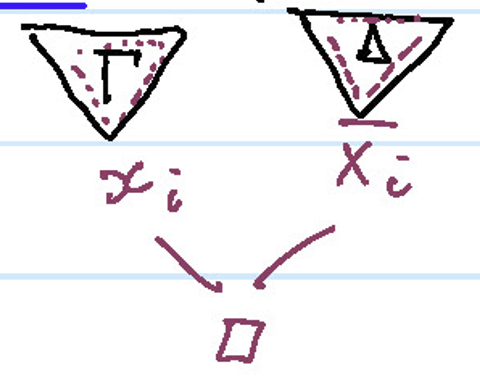
\includegraphics[width=0.2\textwidth]{images/image016.png}

% \[
% \begin{array}{c}
%     A \lor x_i \quad B \lor \neg x_i \\
%     \hline
%     A \lor B
% \end{array}
% \]

(W.l.o.g., assume that $\pi$ is of size $\leq 2^b$.) Then by induction on $b$:

\[
w(F_{x_i := 0} \vdash \square) \leq \log_2(S_T(F_{x_i := 0} \vdash \square)) + w(F) = b - 1 + w(F).
\]

And by induction on $n$:

\[
w(F_{x_i := 1} \vdash \square) \leq \log_2(S_T(F_{x_i := 1} \vdash \square)) + w(F) \leq b.
\]

It suffices now to glue the two proofs together in a way that preserved small width.
This is shown below via inspecting that the glueing lemma we proved in \Cref{lem:glueing-no-width} indeed preserves small width. 
\subsubsection{The Gluing Lemma Preserves Small Width }

We need the following simple structural claims.


\begin{lemma}
The refutation $F_{x_i := 0} \vdash \square$ of width $b - 1 + w(F)$  
and the refutation $F_{x_i := 1} \vdash \square$ of width $b + w(F)$  
can be glued into a refutation of $F$ with width $b + w(F)$.
\end{lemma}

\begin{proof}

\begin{claim}
Assume $F_{x_i := 0} \vdash_{b - 1 + w(F)} \square$, meaning that from $F_{x_i := 0}$ we have a resolution refutation of width $\leq b - 1 + w(F)$. Then, $F \vdash_{b + w(F)} x_i$, meaning there is a resolution derivation of $x_i$ from $F$ of width $\leq b + w(F)$.
\end{claim}

\textbf{Proof of Claim:} 

Consider $F_{x_i := 0} \vdash \square$. By assumption, it has width $b - 1 + w(F)$.

- We are going to turn this refutation from $F_{x_i := 0}$ into a \textbf{derivation} of $x_i$ from $F$ of width $b + w(F)$ (i.e., we add one to the width).  
  This is done by, roughly, adding $\lor x_i$ to each clause in the refutation of $F_{x_i := 0} \vdash \square$.

- \textbf{How do we do this precisely?}  
  Consider three types of clauses in $F$:

  \begin{enumerate}
      \item \textbf{Clauses containing literal $x_i$:}  
      We denote this set of clauses by $F_1$.
      
      \item \textbf{Clauses containing literal $\neg x_i$:}  
      We denote this set of clauses by $F_2$.  
      ($F_1$ is disjoint from $F_2$, because we assume we do not have clauses of the form $C \lor x_i \lor \neg x_i$, since such clauses can be removed without increasing the size.)

      \item \textbf{Clauses without $x_i$ and without $\neg x_i$:}  
      We denote this set of clauses by $F_3$.
  \end{enumerate}
 

Now consider what happens to $F = F_1 \cup F_2 \cup F_3$  
when we assign $x_i := 0$ in $F_{x_i := 0}$:

\begin{enumerate}
    \item A clause in $F_1$ looks like $x_i \lor D$.  
    So in $F_{x_i := 0}$, it turns into $D$.
    
    \item A clause in $F_2$ contains $\neg x_i$.  
    So in $F_{x_i := 0}$, this clause becomes true and is erased.
    
    \item A clause in $F_3$ does not contain the variable $x_i$,  
    so in $F_{x_i := 0}$, it stays the same.
\end{enumerate}

Now we are ready to convert  
\[
F_{x_i := 0} \vdash_{b - 1 + w(F)} \square
\]  
to  
\[
F \vdash_{b + w(F)} x_i
\]  
(i.e., a derivation of the clause $x_i$ from $F$, of width $b + w(F)$).

\begin{center}
        \textbf{Simply add $\lor x_i$ to each clause in $F_{x_i := 0} \vdash_{b - 1 + w(F)} \square$.}
\end{center}
 

It remains to show that doing so turns  
\[
F_{x_i := 0} \vdash_{b - 1 + w(F)} \square \quad \text{into} \quad F \vdash_{b + w(F)} x_i.
\]

\begin{enumerate}
    \item Since we add one variable to each clause, the width is indeed $\leq b + w(F)$.
    
    \item A clause $D$ in $F_{x_i := 0}$ was the clause $D \lor x_i$ in $F$,  
    which, when assigning $x_i = 0$, turned into $D$.  
    Now, when we add $\lor x_i$, we get back to the original clause $D \lor x_i$ in $F$.

    \item A clause $D \lor \neg x_i$ in $F_2$ has disappeared in $F_{x_i := 0}$,  
    so it does not appear in $F_{x_i := 0} \vdash \square$.

    \item A clause $D$ in $F_3$ does not contain $x_i$ or $\neg x_i$.  
    When we add $\lor x_i$ to $D$, we get a new clause not in $F$.  
    But we can derive, using a single \textbf{weakening rule}, the clause $D \lor x_i$.  
    Hence, in every place $D \lor x_i$ appears, we simply add $D$ to the resolution derivation,  
    which turns it into a legal resolution derivation from $F$.
\end{enumerate}

\textbf{ }

\begin{enumerate}
    \item[e)] If in $F_{x_i := 0} \vdash \square$, we used the \textbf{resolution rule}:
    \[
    \frac{A \lor v \quad B \lor w}{A \lor B}
    \]
    for some variable $w \in \{x_1, \dots, x_n\} \setminus \{x_i\}$  
    (\textit{recall that variable $x_i$ does not occur in $F_{x_i := 0}$}),  
    then when adding $\lor x_i$, it turns into a \textbf{legit resolution rule}:

    \[
    \frac{x_i \lor A \lor v \quad x_i \lor B \lor w}{x_i \lor A \lor B}
    \]
\end{enumerate}

\textbf{Illustration of the transformation from $F$ to $F_{x_i := 0}$:}

\begin{center}
    \begin{tabular}{|c|c|c|}
        \hline
        $x_i \in F_1$ & $x_i \in F_2$ & $x_i \notin F$ \\
        \hline
        $(x_i \lor D_1), (x_i \lor D_2), \dots$ & $(\neg x_i \lor C_1), (\neg x_i \lor C_2), \dots$ & Original $F$ \\
        \hline
        $D_1, \dots, D_t$ & Removed & $F_3$ \\
        \hline
    \end{tabular}
\end{center}

\textbf{Conclusion:}  
By the claim, we obtain a resolution derivation $\pi$ of $x_i$ from $F$  
of width $b + w(F)$.


\textbf{ }

Now, we use $F \vdash_{b + w(F)} x_i$ on the clauses of $F$ to get rid (resolve)  
all the literals $\neg x_i$ in $F$.  
This is simple: derive $x_i$ from $F$, and then resolve $D \lor \neg x_i$ in $F$  
by $x_i$ to get $D$.

\textbf{Note} that this way we get a derivation of $F_{x_i := 1}$ from $F$, of width $b + w(F)$.  
This is because $F_{x_i := 1}$ contains precisely all the clauses in $F$ that  
contain neither $x_i$ nor $\neg x_i$ ($F_3$ above), and the clauses $D$  
such that $x_i \lor D$ is in $F$ (i.e., $F_2$ above).  
(The clause $x_i \lor D$ in $F$ gets deleted in $F_{x_i := 1}$.)

By assumption,  
\[
F_{x_i := 1} \vdash_{b + w(F)} \square,
\]
namely, after we derived $F_{x_i := 1}$ from $F$ with a resolution derivation of width $b + w(F)$,  
we derive $\square$, and finish the proof of the theorem.





\mbox{}
\end{proof}
%%%%%%%%%%%%%%%%%%%%%%%%%% Glueing Lemma end of Proof

% 
% \textbf{We need the following simple structural claims.}
% 
% \textbf{Notation:} For a variable $x$ we define $x' := x$ and $x^0 := \neg x$.
% 
%  
% \textbf{Definition (Restriction of a proof/ref):} Let $F$ be a CNF.
% 
% Define $F_{x_i = \epsilon}$, $\epsilon \in \{0,1\}$ as follows:
% 
% For all clauses $C$ in $F$ do:
% \begin{enumerate}
%     \item If $C$ is a clause in $F$ and $x_i^\epsilon \in C$, then delete $C$ from $F$.
%     \item If $x_i^{1-\epsilon} \in C$, then delete the literal $x_i^{1-\epsilon}$ from $C$ (keep $C$).
%     \item Otherwise, do nothing.
% \end{enumerate}
%  
% 
% \textbf{Examples}
% \begin{enumerate}
%     \item 
%     \[
%     \begin{array}{c}
%     (x_1 \lor x_2 \lor x_3) \\
%     \downarrow x_1 = 0 \\
%     (0 \lor x_2 \lor x_3) \\
%     \downarrow \text{(simplified)} \\
%     (x_2 \lor x_3)
%     \end{array}
%     \]
% 
%     \item 
%     \[
%     \begin{array}{c}
%     (x_1 \lor x_2 \lor x_3) \\
%     \downarrow x_1 = 1 \\
%     (1 \lor x_2 \lor x_3) \\
%     \downarrow \text{(delete it, since it's not usable)}
%     \end{array}
%     \]
% \end{enumerate}
% 
% \textbf{Conclusion:} $F \vdash_{x = \epsilon}$ for $\epsilon \in \{0,1\}$  
% assigning $0$ or $1$ in $F$ for $x$  
%where $0,1$ then leads to deletion of literal, clause, respectively.


\section{The Dag-like Refutation Case}


\begin{tcolorbox}[colframe=white, colback=blue!4, boxrule=0mm, sharp corners]
\begin{theorem}[DAG-like Resolution refutation size-width tradeoff~\cite{BSW99}]
Let $F$ be a CNF with $n$ variables and width $w(F) = k$.
Then,  
$$
S(F \vdash \square) \geq 
    2^{
        \Omega
            \left(
                \frac{
                    \left(
                        w(F \vdash \square) - w(F)
                    \right)^2
                    }
                    {n}
            \right)}.
$$
\end{theorem}
\end{tcolorbox}
 

\begin{proof}
It is sufficient to show that
\[
w(F \vdash 0) \leq O\left(\sqrt{n \log(\text{SIZE}_{\text{DAG}}(F \vdash 0))}\right) + k.
\]


 Assume that $\pi$ is the minimal resolution refutation of $F$. Let $|\pi| = s$.

If $s = 1$, then $\square \in F$ and we are  done. We can thus assume  $s > 1$.
\bigskip

\begin{tcolorbox}[colframe=white, colback=red!5, boxrule=0mm, sharp corners,breakable]
\noindent \textbf{Upshot of the argument}:
The idea is to do something similar to the tree-like case above, only that here we cannot recurse by partitioning the tree-like refutation into two \emph{disjoint} sub-refutations, of which one is at most $s/2$: the tree-likeness of the refutation before enabled us to partition the derivation of $\Box$ into two disjoint parts, the first deriving $x_i$ and the second $\neg x_i$, for some $i$. But for a DAG-like refutation there is no guarantee that the these two derivations are disjoint. The solution is to go by induction on the logarithm $b$ of the number of wide clauses, where the base of the logarithm is a number denoted $a$---this $a$ is the factor we are guaranteed to be able to shave off from the number of wide clauses in each induction step. Hence, in $b$ steps we reach the base case of the induction in which the number of wide clauses is zero. Specifically, in each step of the induction we pick the most popular literal within the set of wide clauses, which occurs in at least a $\delta$ fraction of wide clauses. Once we set this literal to 0 or 1, at most $(1-\delta)$ fraction of wide clauses remain. If we set $a=1/(1-\delta)$, it means that in each induction step we multiply the number of wide clauses by $(1-\delta)$ (namely, getting a $(1-\delta)$ fraction of them) means that we shaved off a factor of $a$ for this number. 
\end{tcolorbox}
\bigskip

Let $\pi^*$ be the set of \textit{wide} clauses in $\pi$, meaning that they have more than $d$ literals, for  
$$
    \text{ } d = \sqrt{2n \log s} 
$$
  and let 
    \[
    a = \frac{1}{\left(1 - \frac{d}{2n} \right)}.
    \]
This  $d$ is chosen as to optimise the parameters. Let $b$ be the minimal integer such that $|\pi^*| \leq a^b$.
We prove by (double) induction on $b$ and $n$ that  
    \[
    w(F \vdash 0) \leq d + b + k
    \]
    which concludes the proof by the computations below.

\Base  If $b = 0$, then $|\pi^*| < a^0 = 1$, hence the number of clauses of width at least $d$ is zero, i.e., $w(F\vdash\Box)<d$, and we are done.
 If $n = 1$, then $F$ is either the empty clause, or contains the literals $x_1$ and $\neg x_i$. Thus $k=$ or $k=1$, and  $w(F \vdash 0) \le k$ and we are done.

\induction By an \textit{averaging} argument:  What is the average number a literal, out of the $2n$ literals, occurs in the set $\pi^*$ of wide clauses? Every wide clause has $> d$ literals, and there are $|\pi^*|$ such clauses, so the answer is more than  $\frac{|\pi^*|\cd d}{2n}$. Since, each given literal occurs at most once in a clause, it means that this average number is also the average number of clauses in which each literal occurs. Therefore, there \emph{exists} at least one literal that occurs in $\ge \frac{|\pi^*|\cd d}{2n}$ many clauses. 
Without loss of generality assume that this is a \emph{positive} literal $x_i$.
    
\textit{Eliminate} this literal by setting $x_i = 0$. We get a refutation $\pi\rst_{x_i = 0}$ of $F\rst_{x_i = 0}$ such that:
    \[
    \left|\pi^*\!\!\rst_{x_i = 0}\right| < (a^b) \left( 1 - \frac{d}{2n} \right) = \left( \frac{a^b}{a} \right) = a^{b-1}.
    \]

    \begin{enumerate}
        \item By the induction hypothesis, we thus get
        \[
        w(F\rst_{x_i = 0} \vdash 0) \leq d + b + k - 1.
        \]
        \item By the induction hypothesis, we also have
        \[
        w(F\rst_{x_i = 1} \vdash 0) \leq d + b + k.
        \]
    \end{enumerate}

    Using the gluing lemma, 1 and 2 above imply 
    $w(F \vdash 0) \leq d + b + k$.


\bigskip 
It remains to prove the following:


    \[
    d + b + k \leq O\left(\sqrt{n \log s}\right) + k, \quad \text{for } d = \sqrt{2n \log s}.
    \]
Since $|\pi^*|\le|\pi|$ we have
    \[
    a^b \le s \Rightarrow b \le \log_{a} s = 
    \log_{
        \left(
            \frac{1}{1-\frac{d}{2n}}
        \right)
      }s,
    \]
    from which we get:
    \[
    d + b + k \le d + \log_{\left(\frac{1}{1 - \frac{d}{2n}}\right)}s + k.
    \]
    We use the following simple approximation for $0<\varepsilon<1$ (see below):
    \[
    \frac{1}{1 - \varepsilon} \ge  1 + \varepsilon,
    \]
    to get that $d+b+k$
    \[
    \leq d + \log_{\left(1 + \frac{d}{2n} \right)} s + k.
    \]
We use another simple approximation (see also below):
\[
 \quad \log_{1+\varepsilon} x \ge 2\cd \frac{1}{\varepsilon} \log x,
    \]
(where we use ``$\log x$'' to mean logarithm in the base 2) to get
    \[
    \leq d + O\left(\frac{2n \log s}{d} \right) + k.
    \]
    Substituting $d = \sqrt{2n \log s}$, we have:
    \begin{align*}
    &= \sqrt{2n \log s} + O \left(\frac{2n \log s}{\sqrt{2n \log s}}\right) + k\\
       & = O\left(\sqrt{n \log s} \right) + k.
    \end{align*}
       \mbox{}
\end{proof}

\newcommand{\commentout}[1]{}


\commentout{
       
        **Proof:**
       Using the **change of base formula** for logarithms:
       
       \[
       \log_{1+\varepsilon} x = \frac{\log_2 x}{\log_2 (1+\varepsilon)}.
       \]
       
       Thus, we need to show:
       
       \[
       \frac{\log_2 x}{\log_2 (1+\varepsilon)} \leq \frac{1}{\varepsilon} \log_2 x.
       \]
       
       Dividing both sides by \( \log_2 x \) (which is positive),
       
       \[
       \frac{1}{\log_2(1+\varepsilon)} \leq \frac{1}{\varepsilon}.
       \]
       
       This reduces to proving:
       
       \[
       \log_2 (1+\varepsilon) \geq \varepsilon.
       \]
       
       Justification:**
       For small \(\varepsilon\), we use the first-order **Taylor series expansion**:
       
       \[
       \log_2 (1+\varepsilon) = \frac{\ln(1+\varepsilon)}{\ln 2} \approx \frac{\varepsilon}{\ln 2}.
       \]
       
       -----
       
         why  
       \[
       \ln(1+\varepsilon) \approx \varepsilon \quad \text{for small } \varepsilon.
       \]
       
         **1. Taylor Series Expansion of \( \ln(1+\varepsilon) \)**  
       The **Maclaurin series** for \( \ln(1+\varepsilon) \) around \( \varepsilon = 0 \) is:
       
       \[
       \ln(1+\varepsilon) = \varepsilon - \frac{\varepsilon^2}{2} + \frac{\varepsilon^3}{3} - \frac{\varepsilon^4}{4} + O(\varepsilon^5).
       \]
       
       For **small** values of \( \varepsilon \), the higher-order terms (\( O(\varepsilon^2) \) and beyond) become very small compared to \( \varepsilon \), so the first-order approximation is:
       
       \[
       \ln(1+\varepsilon) \approx \varepsilon.
       \]
       
       This approximation is often called the **first-order Taylor approximation** of \( \ln(1+\varepsilon) \) at \( \varepsilon = 0 \).
       
       ---
       
         **2. Why is this approximation useful?**  
       
       We are dealing with:
       
       \[
       \log_2(1+\varepsilon) = \frac{\ln(1+\varepsilon)}{\ln 2}.
       \]
       
       Substituting the first-order approximation:
       
       \[
       \log_2(1+\varepsilon) \approx \frac{\varepsilon}{\ln 2}.
       \]
       
       Since \( \ln 2 \approx 0.693 \), we can further approximate:
       
       \[
       \frac{\varepsilon}{\ln 2} \approx 1.44 \varepsilon.
       \]
       
       This tells us that for small \( \varepsilon \), \( \log_2(1+\varepsilon) \) behaves approximately linearly with respect to \( \varepsilon \), but with a scaling factor of about \( \frac{1}{\ln 2} \approx 1.44 \).
       
       ---
       
         **3. How Good is this Approximation?**
       We can bound the error by considering the second term in the Taylor expansion:
       
       \[
       \ln(1+\varepsilon) = \varepsilon - \frac{\varepsilon^2}{2} + O(\varepsilon^3).
       \]
       
       For \( 0 < \varepsilon < 1 \), we know that:
       
       \[
       0 < \frac{\varepsilon^2}{2} < \frac{1}{2}.
       \]
       
       Thus, we refine the approximation by writing:
       
       \[
       \varepsilon - \frac{1}{2} \varepsilon^2 \leq \ln(1+\varepsilon) \leq \varepsilon.
       \]
       
       Dividing by \( \ln 2 \), we get:
       
       \[
       \frac{\varepsilon - \frac{1}{2} \varepsilon^2}{\ln 2} \leq \log_2(1+\varepsilon) \leq \frac{\varepsilon}{\ln 2}.
       \]
       
       For \( 0 < \varepsilon < 1 \), the term \( \frac{\varepsilon^2}{2} \) is always **positive**, meaning \( \log_2(1+\varepsilon) \) is actually slightly **less than** \( \frac{\varepsilon}{\ln 2} \). This confirms:
       
       \[
       \log_2(1+\varepsilon) \leq \frac{\varepsilon}{\ln 2}.
       \]
       
       Since \( \frac{1}{\ln 2} \approx 1.44 \), we can further bound:
       
       \[
       \log_2(1+\varepsilon) \leq \frac{\varepsilon}{2},
       \]
       
       which is exactly what we needed in our proof!
       
       ---
       
         **4. Summary**
       - The **first-order Taylor expansion** gives \( \ln(1+\varepsilon) \approx \varepsilon \) for small \( \varepsilon \).
       - This leads to \( \log_2(1+\varepsilon) \approx \frac{\varepsilon}{\ln 2} \).
       - Using a **rigorous bound**, we showed \( \log_2(1+\varepsilon) \leq \frac{\varepsilon}{\ln 2} \), and since \( \frac{1}{\ln 2} \approx 1.44 \), we could choose a **constant** \( c = 2 \) to complete our proof.
       
       ---
       
       Would you like me to clarify any specific part further?
       
       
       -----
       Since \( \ln 2 \approx 0.693 \), we get:
       
       \[
       \log_2(1+\varepsilon) \geq \varepsilon
       \]
       
       for small \( \varepsilon \), meaning the desired inequality **holds**.
       
       Thus,
       
       \[
       \log_{1+\varepsilon} x \leq \frac{1}{\varepsilon} \log_2 x
       \]
       
       is **true** for small \( \varepsilon \).
       
       \
       
       \uline{Second approximation}:Yes! We can prove the required inequality **elementarily** without using pre-established bounds like \( \ln(1+\varepsilon) \leq \varepsilon - \frac{\varepsilon^2}{2} \). Instead, we will rely only on basic properties of logarithms and the Mean Value Theorem (MVT).  
       
       ---
       
         **Step 1: Restating the Problem**
       We want to prove that for \( 0 < \varepsilon < 1 \), there exists a constant \( c \) such that
       
       \[
       \log_{1+\varepsilon} x \geq c \cdot \frac{1}{\varepsilon} \log_2 x.
       \]
       
       Using the change of base formula,
       
       \[
       \log_{1+\varepsilon} x = \frac{\log_2 x}{\log_2 (1+\varepsilon)}.
       \]
       
       Thus, we need to show that:
       
       \[
       \frac{1}{\log_2(1+\varepsilon)} \geq c \cdot \frac{1}{\varepsilon}.
       \]
       
       This is equivalent to proving:
       
       \[
       \log_2(1+\varepsilon) \leq \frac{\varepsilon}{c}.
       \]
       
       We will now prove this for \( c = 2 \), i.e.,
       
       \[
       \log_2(1+\varepsilon) \leq \frac{\varepsilon}{2}.
       \]
       
       for all \( 0 < \varepsilon < 1 \).
       
       ---
       
         **Step 2: Mean Value Theorem on \( \log_2(1+\varepsilon) \)**
       
       Define \( f(x) = \log_2(1 + x) \). Applying the **Mean Value Theorem (MVT)** on \( f(x) \) over the interval \([0, \varepsilon]\), there exists some \( c \in (0, \varepsilon) \) such that:
       
       \[
       \frac{f(\varepsilon) - f(0)}{\varepsilon - 0} = f'(c).
       \]
       
       Since \( f(0) = \log_2(1) = 0 \), we get:
       
       \[
       \frac{\log_2(1+\varepsilon)}{\varepsilon} = f'(c).
       \]
       
       Now, compute \( f'(x) \):
       
       \[
       f'(x) = \frac{1}{(1+x) \ln 2}.
       \]
       
       Thus, for some \( c \in (0, \varepsilon) \),
       
       \[
       \frac{\log_2(1+\varepsilon)}{\varepsilon} = \frac{1}{(1+c) \ln 2}.
       \]
       
       ---
       
         **Step 3: Bounding \( \log_2(1+\varepsilon) \)**
       
       Since \( c \in (0, \varepsilon) \), we have:
       
       \[
       1 + c \leq 1 + \varepsilon.
       \]
       
       Thus,
       
       \[
       \frac{1}{(1+c) \ln 2} \geq \frac{1}{(1+\varepsilon) \ln 2}.
       \]
       
       Using \( \ln 2 \approx 0.693 \), we know that
       
       \[
       \frac{1}{\ln 2} \approx 1.44 \leq 2.
       \]
       
       Therefore,
       
       \[
       \frac{1}{(1+\varepsilon) \ln 2} \leq \frac{1}{2(1+\varepsilon)}.
       \]
       
       Since \( 1+\varepsilon \leq 2 \) for \( 0 < \varepsilon < 1 \), we get:
       
       \[
       \frac{1}{(1+\varepsilon) \ln 2} \leq \frac{1}{2}.
       \]
       
       Thus, from the MVT equation:
       
       \[
       \frac{\log_2(1+\varepsilon)}{\varepsilon} \leq \frac{1}{2}.
       \]
       
       Multiplying by \( \varepsilon \) gives:
       
       \[
       \log_2(1+\varepsilon) \leq \frac{\varepsilon}{2}.
       \]
       
       This is exactly what we needed!
       
       ---
       
         **Step 4: Conclusion**
       Since we have shown
       
       \[
       \log_2(1+\varepsilon) \leq \frac{\varepsilon}{2},
       \]
       
       we substitute this back into our earlier equation:
       
       \[
       \frac{1}{\log_2(1+\varepsilon)} \geq \frac{2}{\varepsilon}.
       \]
       
       Thus,
       
       \[
       \log_{1+\varepsilon} x \geq 2 \cdot \frac{1}{\varepsilon} \log_2 x.
       \]
       
       Choosing \( c = 2 \) proves the required inequality.
       
---

  **Final Answer**
We have **proved elementarily** that for \( 0 < \varepsilon < 1 \),

\[
\log_{1+\varepsilon} x \geq 2 \cdot \frac{1}{\varepsilon} \log_2 x.
\]

Thus, the inequality holds for **constant \( c = 2 \)**. This proof **only used the Mean Value Theorem and elementary bounds**, without relying on any pre-established bounds for \( \ln(1+\varepsilon) \).
} % commentout

% ----------------
% 


% -----------------------------
% Feasible Interpolation for Resolution Refutations
% -----------------------------

\section{Feasible Interpolation for Resolution Refutations}
We describe a different way to obtain resolution refutation size lower bounds via the notion of \emph{Feasible Interpolation}. 

The idea is to take a short resolution refutation of a certain type of unsatisfiable formulas, and convert it to a Boolean circuit computing a certain function. If the function is hard for small Boolean circuits, then we could not have started from a short resolution refutation to begin with. In other words, \emph{there is no short resolution refutation of the unsatisfiable formula}.


\bigskip

\begin{theorem}[Interpolation Theorem]
Let \(\varphi(\mathbf{x},\mathbf{z})\) be a propositional formula over variables \(x_{1},\dots,x_{m}, z_{1},\dots,z_{m}\), and let \(\psi(\mathbf{y},\mathbf{z})\) be a propositional formula over variables \(y_{1},\dots,y_{m}, z_{1},\dots,z_{m}\). 
Suppose that the only shared variables between \(\varphi\) and \(\psi\) are \(\mathbf{z}\). 
Assume that 
\[
\varphi(\mathbf{x},\mathbf{z}) \;\land\; \psi(\mathbf{y},\mathbf{z})
\]
is unsatisfiable.

Then there is a Boolean function 
\[
I \colon \{0,1\}^m \;\to\;\{0,1\}
\]
called the \emph{interpolant} of \(\varphi\) and \(\psi\) such that
\[
\bigl(\varphi(\mathbf{x},\mathbf{z}) \;\land\; I(\mathbf{z})\bigr)
\;\;\lor\;\;
\bigl(\psi(\mathbf{y},\mathbf{z}) \;\land\;\neg I(\mathbf{z})\bigr)
\]
is unsatisfiable.
\end{theorem}

Illustration of the simple argument :

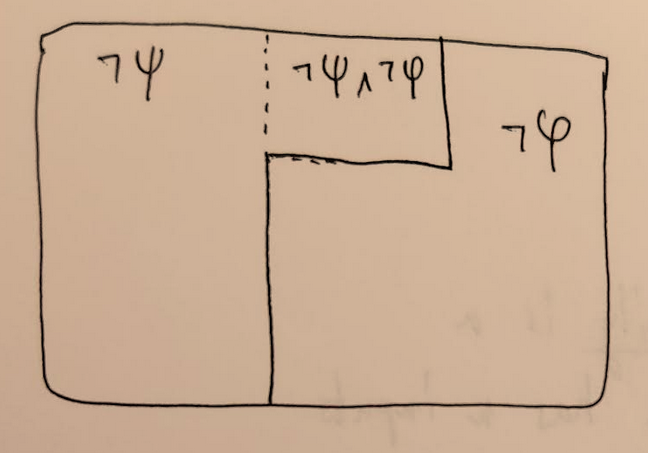
\includegraphics{images/image020.png}
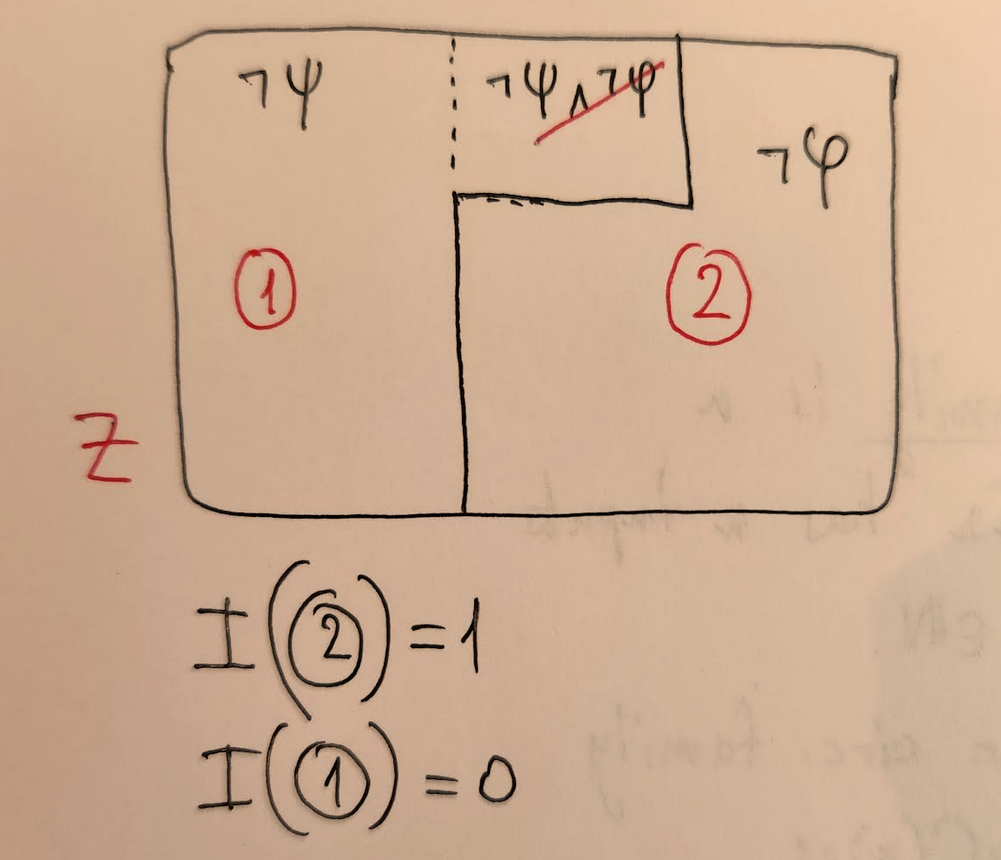
\includegraphics{images/image019.png}



\begin{proof}
For every assignment \(\mathbf{c} \in \{0,1\}^m\), either \(\varphi(\mathbf{x}, \mathbf{c})\) is unsatisfiable or \(\psi(\mathbf{y}, \mathbf{c})\) is unsatisfiable (or both are unsatisfiable). 

 
 
This is because if both \(\varphi(\mathbf{x},\mathbf{c})\) and \(\psi(\mathbf{y},\mathbf{c})\) are satisfiable, then we could combine these two assignments for \(\mathbf{x}\) and \(\mathbf{y}\) (noting that \(\mathbf{x}\) and \(\mathbf{y}\) are disjoint) to obtain a satisfying assignment for \(\varphi \wedge \psi\). Hence \(\varphi \wedge \psi\) would not be unsatisfiable, contradicting our assumption.

\begin{enumerate}[label=\textbf{(\alph*)}]
    \item \textbf{Case 1:} \(\varphi(\mathbf{x},\mathbf{c})\) is satisfiable, which implies \(\psi(\mathbf{y},\mathbf{c})\) must be unsatisfiable. 

    We define \( I(\mathbf{c}) := 0\). Then observe that
    \[
      \bigl(\underbrace{\overbrace{\varphi(\mathbf{x},\mathbf{c})}^{\rm satisfiable} \;\land\; \underbrace{I(\mathbf{c})}_{0}}_0\bigr)
      \;\;\lor\;\;
      \bigl(\overbrace{\psi(\mathbf{y},\mathbf{c}) }^{\rm unsatisfiable}\;\land\;\underbrace{\neg I(\mathbf{c})}_1\bigr)
    \]
    is unsatisfiable. 
    %(1)

    \item \textbf{Case 2:} Otherwise, \(\varphi(\mathbf{x},\mathbf{c})\) is unsatisfiable. We then set \(I(\mathbf{c}) := 1\). Hence
    \[
      \bigl(\varphi(\mathbf{x},\mathbf{c}) \;\land\; I(\mathbf{c})\bigr)
      \;\;\lor\;\;
      \bigl(\psi(\mathbf{y},\mathbf{c}) \;\land\;\neg I(\mathbf{c})\bigr)
    \]
    is unsatisfiable.

\end{enumerate}

\noindent
Therefore, \(I\) is well-defined completing the construction of the interpolant.
\end{proof}


\begin{theorem}
[Interpolation Theorem for Resolution]
\label{thm:interpolation-circuit}
In the setting of the previous theorem, suppose 
\(\varphi(\mathbf{x},\mathbf{z}) \wedge \psi(\mathbf{y},\mathbf{z})\) 
admits a resolution refutation of size \(s\). Then there is an interpolant function 
\[
I \colon \{0,1\}^m \to \{0,1\}
\]
that can be computed by a Boolean circuit of size \(O(s^2)\).

Furthermore, if the variables \(\mathbf{z}\) appear all in \emph{positive} form in 
\(\psi(\mathbf{y},\mathbf{z})\), then the above circuit is \emph{monotone}. 
Similarly, if all \(\mathbf{x}\) variables in \(\varphi(\mathbf{x},\mathbf{z})\) 
appear in \emph{negative} form, the resulting circuit is also monotone.
\end{theorem}

Applying this theorem to derive a resolution refutation lower bound is now straightforward, as we can argue that any short resolution refutation would yield a small circuit for a function believed to be hard, leading to a contradiction.

\begin{theorem}[Lower bounds on resolution refutations of the CLIQUE--COLOURING principle]\label{thm:interpolation-lower-bound}
Let us define the following unsatisfiable CNF formulas \(\varphi_n(\mathbf{x},\mathbf{z})\) and \(\psi_n(\mathbf{y},\mathbf{z})\). Intuitively,
\[
\varphi_n(\mathbf{x},\mathbf{z}) = 1 \quad\text{iff}\quad \mathbf{x} \text{ encodes a }\sqrt[4]{n}\text{-clique in the graph on }n\text{ nodes represented by }\mathbf{z}.
\]
\[
\psi_n(\mathbf{y},\mathbf{z}) = 1 \quad\text{iff}\quad \mathbf{y} \text{ encodes a }(\sqrt[4]{n}-1)\text{-colouring of that same graph.}
\]
Then 
\[
\varphi_n(\mathbf{x},\mathbf{z}) \;\wedge\; \psi_n(\mathbf{y},\mathbf{z})
\]
is unsatisfiable, and the smallest resolution refutation of \(\varphi_n \wedge \psi_n\) has size at least
\[
2^{\,c\sqrt[8]{n}}
\]
for some constant \(c>0\).
\end{theorem}

\medskip
\noindent
\textbf{Note:} Indeed, \(\varphi_n \wedge \psi_n\) is unsatisfiable because no graph on \(n\) nodes can simultaneously contain a \(\sqrt[4]{n}\)-clique and admit a \((\sqrt[4]{n}-1)\)-colouring.

\medskip

To be precise, we now show how to encode 
$ \varphi_n(\mathbf{x},\mathbf{z}) \;\wedge\; \psi_n(\mathbf{y},\mathbf{z})$ formally, with a CNF of total size \(O(n^2)\) size, ensuring that all \(\mathbf{z}\) variables appear \emph{positively} in \(\varphi_n\) and \emph{negatively} in \(\psi_n\).
This formulation is taken from Raz-Tzameret \cite{RT07}. 




Let $G=(V,E)$ be an undirected graph with $n$ vertices and let $k'<k$ be
two integers.
Then, one of the following must hold:
\begin{description}
\item[(i)] The graph $G$ does not contain a \emph{clique with $k$ vertices};

\item[(ii)] The graph $G$ is not a \emph{complete $k'$-partite graph}.
In other words, there is no way to partition $G$ into $k'$ subgraphs
$G_1\dots G_{k'}$,
such that every $G_i$ is an independent set, and for all $i\ne j \in[k']$,
all the vertices in $G_i$ are connected by edges (in $E$) to all the vertices in $G_j$.
\end{description}

Obviously, if Item (ii) above is false
(that is, if $G$ is a complete $k'$-partite graph),
then there exists a $k'$-coloring of
the vertices of $G$; hence the name \emph{clique-coloring} for the principle.

The propositional formulation of the (negation of the)
clique-coloring principle is as follows.
Each variable $z_{ij}$, for all $i\ne j \in [n]$,
is an indicator variable for the fact that there is an edge in $G$
between vertex $i$ and vertex $j$.
Each variable $x_{\ell i}$, for all $\ell\in[k]$ and all $i\in[n]$,
is an indicator variable for the fact that the vertex $i$ in $G$
is the $\ell$th vertex in the $k$-clique.
Each variable $ y_{\ell i}$, for all $\ell\in[k']$ and all $i\in[n]$,
is an indicator variable for the fact that the vertex $i$ in $G$
pertains to the independent set $G_\ell$.

\begin{definition}\label{def-clique-color}
The negation of the clique-coloring principle consists of the following
unsatisfiable collection of clauses:

$\varphi_n(\mathbf{x,z})$:
\renewcommand{\theenumi}{\roman{enumi}}   % change temporarily to Roman items
\begin{enumerate}
\item $x_{\ell,1}\lor\dots\lor x_{\ell,n}, \mbox{ for all } \ell\in[k]$

(expresses that there exists at least one vertex in $G$ which constitutes
the $\ell$th vertex of the $k$-clique); \label{eq-clique-q-pigeons}%\vspace{-6pt}

\item $\neg x_{\ell,i}\lor \neg x_{\ell,j},  \mbox{ for all } i\ne j \in [n],\;
          \ell\in[k]$

(expresses that there exists at most one vertex in $G$ which constitutes
the $\ell$th vertex of the $k$-clique); \label{eq-clique-functional-q}%\vspace{-6pt}

\item $\neg x_{\ell,i}\lor \neg x_{\ell',i}, \mbox{ for all } i\in [n],\;
          \ell\ne \ell'\in[k]$

(expresses that the $i$th vertex of $G$ cannot be both the $\ell$th
and the $\ell'$th vertex of the $k$-clique);\label{eq-clique-holes-q}%\vspace{-6pt}

\item $\neg x_{\ell,i}\lor \neg x_{\ell',j}\lor z_{i,j}, \mbox{ for all }
\ell\ne\ell'\in[k], i\ne j\in[n]$

(expresses that if both the vertices $i$ and $j$ in $G$ are in the $k$-clique,
then there is an edge in $G$ between $i$ and $j$).
\label{eq-clique-p-and-q-vars}%\vspace{-6pt}
\end{enumerate}

$\psi_n(\mathbf{y},\mathbf{z})$:

\begin{enumerate}


\item $y_{1,i}\vee \dots \vee y_{k',i}, \mbox{ for all } i\in[n]$

(expresses that every vertex of $G$ pertains to at least one independent set);
\label{eq-clique-r-pigeons}%\vspace{-6pt}

\item  $\neg y_{\ell,i}\lor \neg y_{\ell',i}, \mbox{ for all } \ell\ne\ell\in[k'], i\in[n]$

(expresses that every vertex of $G$ pertains to at most one independent set);
\label{eq-clique-holes-r}%\vspace{-6pt}

\item $\neg z_{i,j}\lor \neg y_{t,i}\lor \neg y_{t,j}, \mbox{ for all } i\ne j\in[n],
t\in[k']$

(expresses that if there is an edge between vertex $i$ and $j$ in $G$, then
$i$ and $j$ cannot be in the same independent set);
\label{eq-clique-final-contradictory-clauses}
\end{enumerate}
\renewcommand{\theenumi}{(\Roman{enumi})}   % change back to Roman items
\end{definition}



\begin{proof}[of \Cref{thm:interpolation-lower-bound}]
By the feasible interpolation theorem, if there exists a resolution refutation of 
\(\varphi_n(\mathbf{x},\mathbf{z}) \;\wedge\; \psi_n(\mathbf{y},\mathbf{z})\)
of size smaller than \(2^{c\sqrt[8]{n}}\) (for sufficiently small \(c\)), then there is an interpolant 
\[
I_n : \{0,1\}^{n \choose 2} \;\longrightarrow\; \{0,1\}
\]
for \(\varphi_n \wedge \psi_n\) that can be computed by a \emph{monotone} circuit of size less than \(2^{2\,c\sqrt[8]{n}}\).

But this interpolant \(I_n\) then decides the function 
\(\textsc{CLIQUE}(n,\sqrt[4]{n})\), thus contradicting the monotone circuit lower bound we proved earlier!

\medskip

\noindent
\textbf{Why does \(I_n\) compute \(\textsc{CLIQUE}(n,\sqrt{n})\)?}
Consider the ``extreme'' positive or negative assignments to \(\mathbf{z}\). By definition:
\begin{enumerate}[label=\textbf{(\alph*)}]
    \item If \(I_n(\mathbf{z}) = 1\), then \(\varphi_n(\mathbf{x},\mathbf{z})\) is unsatisfiable.
    \item If \(I_n(\mathbf{z}) = 0\), then \(\varphi_n(\mathbf{x},\mathbf{z})\) is satisfiable, which forces \(\psi_n(\mathbf{y},\mathbf{z})\) to be unsatisfiable.
\end{enumerate}

Thus, for \(\mathbf{z}\) that encodes either a \(\sqrt[4]{n}\)-clique or a \((\sqrt[4]{n}-1)\)-colouring in the underlying graph,
\[
I_n(\mathbf{z}) = 
\begin{cases}
1, & \text{if }\mathbf{z}\text{ encodes a }(\sqrt[4]{n}-1)\text{-colouring},\\
0, & \text{if }\mathbf{z}\text{ encodes a }\sqrt[4]{n}\text{-clique}.
\end{cases}
\]
Hence \(I_n\) distinguishes between \(\sqrt[4]{n}\)-cliques and \((\sqrt[4]{n}-1)\)-colourings, which is exactly the \(\textsc{CLIQUE}(n,\sqrt{n})\) function, contradicting the known monotone circuit lower bound. 
\end{proof}

\bigskip 


\begin{proof}[of \Cref{thm:interpolation-circuit}]
Given an assignment \(\mathbf{c} \in \{0,1\}^m\), we explain how to compute \(I(\mathbf{c})\) by transforming a size-\(s\) resolution refutation of
\[
\varphi(\mathbf{x},\mathbf{z}) \;\wedge\; \psi(\mathbf{y},\mathbf{z})
\]
into a refutation of either \(\varphi(\mathbf{x}, \mathbf{c})\) (meaning \(\varphi(\mathbf{x}, \mathbf{c})\) is unsatisfiable, so \(I(\mathbf{c}) = 1\)) or \(\psi(\mathbf{y}, \mathbf{c})\) (meaning \(I(\mathbf{c}) = 0\)). We accomplish this in time \(O(s^2)\).
Since this algorithm is computed in time $O(s^2)$ there is also a Boolean circuit, that by inspection of the algorithm is also a monotone one. 



\paragraph{Size of the new refutation}
The resulting refutation has size \(O(s)\). Concretely, we take the original resolution refutation and, using the assignment \(\mathbf{c}\), \emph{discard} all \(\mathbf{z}\) variables from every clause in the proof. By doing so, we obtain a refutation of
\[
\varphi(\mathbf{x},\mathbf{c}) \;\wedge\; \psi(\mathbf{y},\mathbf{c}),
\]
which must end in a contradiction.

\paragraph{Maintaining the structure}
We ensure that each clause in the modified refutation:
\begin{enumerate}
\item 
  contains \emph{only} \(\mathbf{x}\)-variables or \emph{only} \(\mathbf{y}\)-variables; and 

\item  is derived correctly from previous (already modified) clauses, or is an axiom; and

\item we do not remove $\overline x$-variables 
 from $\overline x$-clauses and  
we do not remove $\overline y$-variables 
 from $\overline y$-clauses.
 
\end{enumerate}

Symbolically, we map every original clause
\[
C_i \quad\longmapsto\quad \widetilde{C_i},
\]
where \(\widetilde C_i\) is the version of \(C_i\) with all \(\mathbf{z}\) variables removed, leaving either only \(\mathbf{x}\) or only \(\mathbf{y}\).

\paragraph{Conclusion}
Since the final line \(\widetilde C_m\) in the refutation is false (denoted by \(\Box\)), and by induction statement is derived correctly from previous clauses, we derive a contradiction in either \(\varphi(\mathbf{x}, \mathbf{c})\) or \(\psi(\mathbf{y}, \mathbf{c})\). 







\paragraph{Inductive Argument on Resolution Refutation Length.}

\noindent
\textbf{Base Case:} 
Every axiom clause in \(\varphi(\overline{x}, \overline{c})\) or \(\psi(\overline{y}, \overline{c})\) is already an \(\overline{x}\)-clause or a \(\overline{y}\)-clause (i.e., it contains only \(\overline{x}\) variables or only \(\overline{y}\) variables).

\medskip

\noindent
\textbf{Induction Step:} 
Suppose \(C_1, \dots, C_{j-1}\) have already been transformed so that each is an \(\overline{x}\)-clause or a \(\overline{y}\)-clause, yielding transformed clauses \(\widetilde{C_1}, \dots, \widetilde{C_{j-1}}\). Now assume the next derived clause 
\[
C_j \;=\; C \;\lor\; D
\]
came from two prior clauses:
\[
C' \;=\; w \;\lor\; C
\quad\quad\text{and}\quad\quad
D' \;=\; \neg w \;\lor\; D
\]
by a resolution step.
By the induction hypothesis, we already have transformed versions \(\widetilde{C'}, \widetilde{D'}\), each of which is either an \(\overline{x}\)-clause or a \(\overline{y}\)-clause. We consider three cases:

\begin{description}
\item[Case 1:] 
\(\widetilde{C'}, \widetilde{D'}\) are both \(\overline{x}\)-clauses. Then \(w\) must be an \(\overline{x}\)-variable common to both (because we maintain the invariant that we do not remove $\overline x$-variables from $\overline x$-clauses or $\overline y$-variables from $\overline y$-clauses). We thus apply the usual resolution rule on \(\widetilde{C'}, \widetilde{D'}\).

\item[Case 2:]
\(\widetilde{C'}, \widetilde{D'}\) are both \(\overline{y}\)-clauses. This is analogous to Case 1, but with a \(\overline{y}\)-variable \(w\).

\item[Case 3:]
\(\widetilde{C'}\) is an \(\overline{x}\)-clause, whereas \(\widetilde{D'}\) is a \(\overline{y}\)-clause, or vice versa. In this scenario, \(w\) must be a \(\overline{z}\)-variable. According to the assignment \(\overline{c}\), we fix the value of \(w\) (it cannot be in \(\overline{x}\) or \(\overline{y}\), so it must be in \(\overline{z}\)). If \(w = 0\), we  define \(\widetilde{C_j} := \widetilde{C'}\). 
If \(w = 1\), we set \(\widetilde{C_j} := \widetilde{D'}\).


% 
% \item[Case 4:]
% \(\widetilde{C'}\) is a \(\overline{y}\)-clause, whereas \(\widetilde{D'}\) is an \(\overline{x}\)-clause. Similarly to Case 3, \(w\) must be a \(\overline{z}\)-variable and according to the assignment \(\overline{c}\), we fix the value of \(w\). If \(w = 0\), we  define \(\widetilde{C_j} := \widetilde{C'}\). 
% If \(w = 1\), we set \(\widetilde{C_j} := \widetilde{D'}\).

\end{description}

\noindent
%In each case, the transformed clause \(\widetilde{C_j'} = \widetilde{C} \lor \widetilde{D}\) remains an \(\overline{x}\)-clause or \(\overline{y}\)-clause or is made into a contradiction (if the variable assignments lead to \(\Box\)). Thus, by induction, all clauses in the resolution refutation can be converted into either \(\overline{x}\)- or \(\overline{y}\)-clauses, completing the step.




\medskip
Note that the last line \(C_m\) of the original resolution refutation is \(\Box\) (i.e.\ false). Hence in our new refutation (possibly ending earlier than the \(m\)-th clause), we must also reach \(\Box\). Starting from the axioms, we obtain a refutation of either \(\varphi(\overline{x},\overline{c})\) or \(\psi(\overline{y},\overline{c})\). 
Thus, the proof concludes with the desired contradiction in one of these formulas. 


\bigskip 

To prove that the same algorithm can be implemented with a \emph{monotone} circuit in case the $\overline z$-variables all appear positive in $\psi$ or they all appear negative in $\varphi$, we notice the following:\ For every index \(j\), let \(d_j(\mathbf{c}) = 0\) if the \(j\)-th clause \(\widetilde{C_j}\) in the modified refutation can be derived using only the \(\mathbf{y}\) variables. It is possible to show that 
 each \(d_j(\mathbf{c})\) can be computed by a monotone circuit of size \(O(s^2)\) in the variables \(\mathbf{c}\).

Observe that \(I(\mathbf{c}) = d_m(\mathbf{c})\), namely $I(\mathbf c)$ is zero only if  $\psi(\mathbf y,\mathbf c)$ is unsatisfiable, and otherwise it is 1, as desired. 
\end{proof}


